\documentclass[12pt,letterpaper,noanswers]{exam}
\usepackage[usenames,dvipsnames,svgnames,table]{xcolor}
\usepackage[margin=0.9in]{geometry}
\renewcommand{\familydefault}{\sfdefault}
\usepackage{multicol}
\pagestyle{head}
\header{AM 108 Class 29}{}{Functionals + 2D maps}
\runningheadrule
\headrule
\usepackage{graphicx} % more modern
\usepackage{amsmath} 
\usepackage{amssymb} 
\usepackage{hyperref}
\usepackage{tcolorbox}

\begin{document}
 \pdfpageheight 11in 
  \pdfpagewidth 8.5in

\noindent 




\begin{itemize}
\itemsep0em
\item You have a project weekly log due Friday (and again next Friday).  Your project work is replacing the problem set.
\item There is a new skill check for Wednesday.
\item The Quiz 02 Follow Up is due Mon Nov 23rd.  The retake, if assigned to you, is due Thurs Dec 3rd.  Request a different due date via private message on Piazza, if needed.
\item There is a pre-class assignment for Wednesday.  \emph{I'm sorry I didn't properly release it for today!}
\end{itemize}

\hrule
\vspace{0.2cm}



\noindent\textbf{Teams}



\noindent \textbf{Teams 1 and 2}: Post screenshots of your work to the course Google Drive today.  Include words, labels, and other short notes that might make those solutions useful to you or your classmates.  Find the link in Canvas (or here: \url{https://drive.google.com/drive/u/0/folders/1GcpwvKHD4tMecpFQ4lNxN_r5Ylj7YHbd})


\vspace{0.2cm}

\hrule
\vspace{0.2cm}


\noindent\textbf{Big picture}

Functional equations are equations to which the solution is a function.  We will introduce them today.

\vspace{0.2cm}
\hrule
\vspace{0.2cm}

\noindent \textbf{Extra vocabulary / extra facts:}
\begin{tcolorbox}
An equation where the function is the unknown is called a \textbf{functional equation}.  For example: $f(x+y) = f(x)f(y)$.  

Given an unknown function, $x(t)$, a \textbf{initial condition} specifies the value of the function (or the value of its derivative) at time $0$. 

For an unknown function of $x$, we use a different term: given an unknown function $f(x)$, a \textbf{boundary condition} specifies the value of the function (or the value of its derivative) at selected points.  These values are referred to as \textbf{boundary values}.
\end{tcolorbox}

\noindent\textbf{Example:}

Consider the functional equation $f(x+y) = f(x)f(y)$.

\begin{enumerate}
\itemsep0em
    \item $0 = 0+0$, so $f(0) = f(0+0) = f(0)f(0)$.  Let $a = f(0)$.  We have $a^2 - a = 0$ so $a = 0$ or $a = 1$.
    \item Try $a = 0$.  We are now solving the problem $f(x+y) = f(x)f(y), f(0) = 0$ (we have added a boundary condition).  $f(x+0) = f(x)f(0) = f(x)(0) = 0$, so we find $f(x) = 0$.  This is one solution to the functional equation.
    \item We'll look at the $f(0) = 1$ case in the problems below.
\end{enumerate}

\vspace{0.2cm}
\hrule
\vspace{0.2cm}

\noindent \textbf{Extra vocabulary / extra facts:}
\begin{tcolorbox}
When we worked with systems of differential equations, trajectories \textbf{could not merge}.

For the logistic map given by $x_{n+1} = 3 x_n(1-x_n)$, the orbit of $x_0 = \frac{1}{2} - \sqrt{6}/6$ and the orbit of $x_0 = \frac{1}{2}+\sqrt{6}/6$ \textbf{do merge}.  This happens because $f(x) = 3x(1-x)$ is not a one-to-one function.

It is possible to create a map where orbits do not merge.  Such a map might be a better model than the logistic map for the dynamics of a system of differential equations.
\end{tcolorbox}

\textbf{Example} orbits do not merge in the Baker's map:

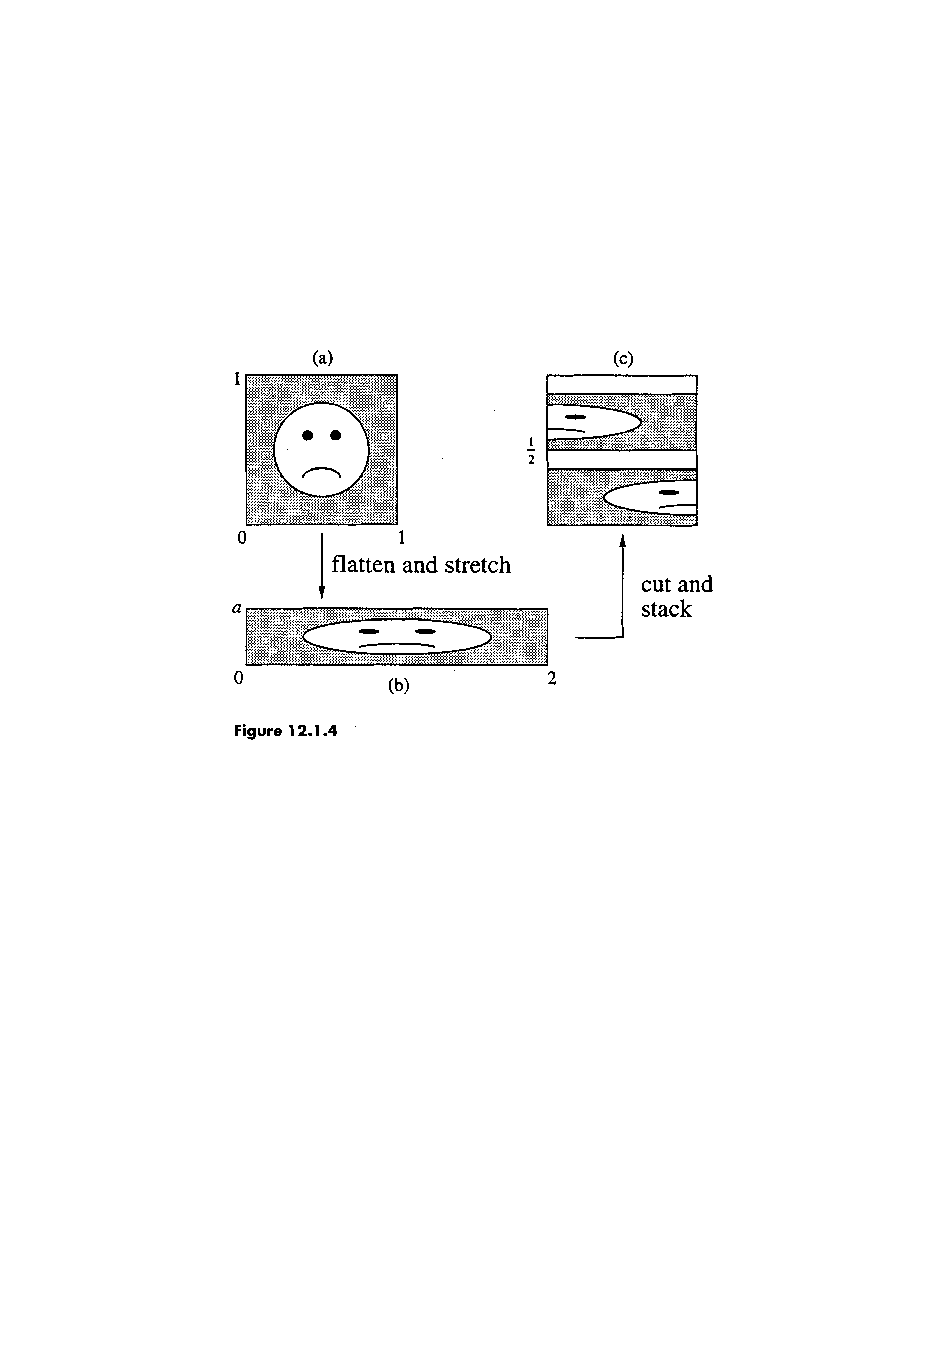
\includegraphics[scale=1]{img/C25baker.pdf}

\vspace{0.2cm}
\hrule
\vspace{0.2cm}

\noindent\textbf{Skill Check C30 practice}
\begin{questions}
\item No retake (there was no skill check for class 27).

\item Consider the functional equation $f(xy) = f(x) + f(y)$.  Use $1 = 1*1$ to find a value for $f(1)$.
\end{questions}

\vspace{0.2cm}

\hrule
\vspace{0.2cm}

\noindent\textbf{Skill Check C30 Practice Solution}

We have $f(1) = f(1*1) = f(1)+f(1) = 2f(1)$ so $f(1) = 2f(1) \Rightarrow f(1) = 0$.


\vspace{0.2cm}

\hrule
\vspace{0.2cm}


\noindent\textbf{Questions}

\noindent \ \ 0.  Share a book or article you found interesting with your team, and write your names on the slide.

\begin{questions}
 \question Let $f(x+y) = f(x)f(y)$.  Choose $f(0) = 1$. 

We have $f(0)=f(x-x) = f(x)f(-x) = 1$ so $f(-x) = f(x)^{-1}$.

Assume $f(1) = a$ (with $a$ positive).



\begin{parts}
\item Find $f(2)$.
\item Find $f(n)$ for $n$ an integer.
\item Find $f(1/2)$.
\item Find $f(p/q)$ for $p$ and $q$ positive integers.
\end{parts}

\question (12.1.1: uncoupled linear map).  Consider the linear map $x_{n+1} = ax_n$, $y_{n+1} = by_n$ where $a, b$ are real parameters.  The origin is a fixed point.

\begin{parts}
\part Draw the possible patterns of orbits near the origin.  Different combinations of signs and sizes of $a$ and $b$ will lead to different patterns.

\emph{Perhaps start at $(1,1)$ and draw the orbit of that point for the different cases that you identify.  There are 16 cases.}
\part Under what conditions is the fixed point stable?
\end{parts}

\question (Practice with changing variables in a function) 

Given a map $y_{n+1} = f(y_n)$, rewrite the map in terms of a rescaled variable, $x_n = \alpha y_n$.  Doing this change of variables, show that $y_{n+2} = f^2(y_n)$ becomes $x_{n+2} = \alpha f^2(x_n/\alpha)$.

\question Consider the functional equation $g(x) = \alpha g^2(x/\alpha)$ with boundary conditions $g'(0) = 0$ and $g(0) = 1$.

\emph{We will work more with this functional equation in the next class.}

\begin{parts}
\part Consider $x=0$ in the functional equation.  Using your boundary condition for $g(0)$ to find an expression for $\alpha$.
\part Let $h(x) = \mu g(x/\mu)$.  Show that if a function $g(x)$ solves the functional equation, so would $h(x)$.
\end{parts}

\end{questions}

\eject

\noindent
1a: $f(2) = f(1)f(1) = a^2$.  

\noindent
1b: $f(n) = f((n-1)+1) = f(n-1)f(1) = af(n-1) = a^n$.  

\noindent
1c: $f(1) = f(1/2+1/2) = f(1/2)^2$ so $f(1/2) = \sqrt{a}$. 

\noindent
1d: $f(p/q) = f(1/q+1/q+...+1/q)= f(1/q)^p.$. $f(q/q) = f(1/q)^q = a$ so $f(p/q) = a^{p/q}$.

\noindent
2:

$x_0=(1,1)$, $x_1 = (a,b)$, $x_2 = (a^2,b^2)$, ..., $x_n = (a^n,b^n),$...
    Cases: $a<-1$, $-1<a<0$, $0<a<1$, $a<1$ are the four cases for $a$.  There are a matching four for $b$, so there are 16 total combinations.
    
    \begin{tabular}{|r | p{3cm}| p{3cm} |p{3cm} |p{3cm}|}
    \hline
    & $a<-1$ & $-1<a<0$ & $0<a<1$ & $1<a$ \\
    \hline
    $b<-1$ & both oscillate and diverge & $x_n\rightarrow 0$, $y_n$ diverges (both oscillate)& $x_n\rightarrow 0$ monotonically, $y_n$ diverges an oscillates & $x_n \rightarrow \infty$, $y_n$ diverges and oscillates\\
    \hline
        $-1<b<0$ & & & &\\
        \hline
            $0<b<1$ & & & &\\
            \hline
                $1<b$ & & & &\\
                \hline
    \end{tabular}
    


\noindent
3: $y_{n+2} = f(y_{n+1}).$. $x_{n+2} = \alpha f( x_{n+1}/\alpha)$.  $x_{n+1} = \alpha f( x_{n}/\alpha).$. So $x_{n+2} = \alpha f( \alpha f( x_{n}/\alpha)/\alpha) = \alpha f^2(x_n/\alpha)$.

\noindent
4a: $g(0) = 1 = \alpha g^2(0/\alpha) = \alpha g(g(0)) = \alpha g(1).$  $1 = \alpha g(1)$, so $\alpha = 1/g(1)$.

4b: Assume $g$ solves the functional equation.  Consider $\mu g(x/\mu)$.  Using the functional equation on $g(x/\mu)$, we have $g(x/\mu) = \alpha g(g(x/\mu/\alpha))$. Multiplying by $\mu$, this is $h(x) = \alpha\mu g(\frac{1}{\mu}\mu g(x/\mu/\alpha))$ so $h(x) = \alpha\mu g(h(x/\alpha)/\mu) = \alpha h(h(x/\alpha)$.

\end{document}